\section{Iterative Bayesian Unfolding}
\label{app:IBU}

As a cross-check and comparison, % bin-by-bin unfolding as well as
Iterative Bayesian Unfolding (IBU) (described in section~\ref{sec:UnfoldIntro}) using the \texttt{RooUnfold} package~\cite{Adye:2011gm} was performed. At present, this uses the information from the \powheg+\pythia~samples to unfold the reconstructed events from the \sherpa~2.2.1 samples, analogous to what has been done with OmniFold up to this point.
%Various plots for the efficiency and purity of the \powheg+\pythia~sample can be found in section~\ref{}, and some comments on the efficiency can be found in section~\ref{}. Finally, the unfolded distributions can be found in section~\ref{}.

First, various plots for the efficiency and purity of the \powheg+\pythia~sample are shown, and the results of the unfolding are shown in the following section.

\subsection{Relevant quantities and choice of binning}
The efficiency describes the probability that an event is reconstructed given that a truth event occurs. This can be written as,
\begin{equation}
  % E=\frac{N({\text{truth | reco}})}{N({\text{truth}})}
  E=\frac{N^{\text{truth$_i$, reco}}}{N^{\text{truth$_i$}}}
\end{equation}

where $i$ is the truth bin. The purity describes the probability that a reconstructed event has a matching truth event. This can be written as,
\begin{equation}
  % P=\frac{N({\text{reco | truth}})}{N({\text{reco}})}
  P=\frac{N^{\text{reco$_i$, truth}}}{N^{\text{reco$_i$}}}
\end{equation}
where $i$ is the reconstructed bin.

Figure~\ref{fig:Eff1} and~\ref{fig:Eff2} shows the efficiency measurements for the 16 variables that were outlined for UniFold and MultiFold, and figure~\ref{fig:Pur1} and~\ref{fig:Pur2} shows the purity for the same variables.

\begin{figure}[h!]
  \centering
  \includegraphics[page=533,width=0.45\textwidth]{figures/UnfoldingRelatedPlots.pdf}
  \includegraphics[page=539,width=0.45\textwidth]{figures/UnfoldingRelatedPlots.pdf} \\
  \includegraphics[page=587,width=0.45\textwidth]{figures/UnfoldingRelatedPlots.pdf}
  \includegraphics[page=629,width=0.45\textwidth]{figures/UnfoldingRelatedPlots.pdf} \\
  \includegraphics[page=593,width=0.45\textwidth]{figures/UnfoldingRelatedPlots.pdf}
  \includegraphics[page=635,width=0.45\textwidth]{figures/UnfoldingRelatedPlots.pdf} \\
  \includegraphics[page=671,width=0.45\textwidth]{figures/UnfoldingRelatedPlots.pdf}
  \includegraphics[page=677,width=0.45\textwidth]{figures/UnfoldingRelatedPlots.pdf}
  \caption{Efficiency measurements for $p_{\text{T},\ell\ell}$, $y_{\ell\ell}$, and $\pt$, $y$, and $N_{cons}$ for the leading and subleading track jets.}
  \label{fig:Eff1}
\end{figure}

\begin{figure}[h!]
  \centering
  \includegraphics[page=605,width=0.45\textwidth]{figures/UnfoldingRelatedPlots.pdf}
  \includegraphics[page=647,width=0.45\textwidth]{figures/UnfoldingRelatedPlots.pdf} \\
  \includegraphics[page=611,width=0.45\textwidth]{figures/UnfoldingRelatedPlots.pdf}
  \includegraphics[page=653,width=0.45\textwidth]{figures/UnfoldingRelatedPlots.pdf} \\
  \includegraphics[page=617,width=0.45\textwidth]{figures/UnfoldingRelatedPlots.pdf}
  \includegraphics[page=659,width=0.45\textwidth]{figures/UnfoldingRelatedPlots.pdf} \\
  \includegraphics[page=623,width=0.45\textwidth]{figures/UnfoldingRelatedPlots.pdf}
  \includegraphics[page=665,width=0.45\textwidth]{figures/UnfoldingRelatedPlots.pdf}
  \caption{Efficiency measurements for $m$, $\tau_1$, $\tau_2$, and $\tau_3$ for the leading and subleading track jet.}
  \label{fig:Eff2}
\end{figure}

\begin{figure}[h!]
  \centering
  \includegraphics[page=534,width=0.45\textwidth]{figures/UnfoldingRelatedPlots.pdf}
  \includegraphics[page=540,width=0.45\textwidth]{figures/UnfoldingRelatedPlots.pdf} \\
  \includegraphics[page=588,width=0.45\textwidth]{figures/UnfoldingRelatedPlots.pdf}
  \includegraphics[page=630,width=0.45\textwidth]{figures/UnfoldingRelatedPlots.pdf} \\
  \includegraphics[page=594,width=0.45\textwidth]{figures/UnfoldingRelatedPlots.pdf}
  \includegraphics[page=636,width=0.45\textwidth]{figures/UnfoldingRelatedPlots.pdf} \\
  \includegraphics[page=672,width=0.45\textwidth]{figures/UnfoldingRelatedPlots.pdf}
  \includegraphics[page=678,width=0.45\textwidth]{figures/UnfoldingRelatedPlots.pdf}
  \caption{Purity measurements for $p_{\text{T},\ell\ell}$, $y_{\ell\ell}$, and $\pt$, $y$, and $N_{cons}$ for the leading and subleading track jets.}
  \label{fig:Pur1}
\end{figure}

\begin{figure}[h!]
  \centering
  \includegraphics[page=606,width=0.45\textwidth]{figures/UnfoldingRelatedPlots.pdf}
  \includegraphics[page=648,width=0.45\textwidth]{figures/UnfoldingRelatedPlots.pdf} \\
  \includegraphics[page=612,width=0.45\textwidth]{figures/UnfoldingRelatedPlots.pdf}
  \includegraphics[page=654,width=0.45\textwidth]{figures/UnfoldingRelatedPlots.pdf} \\
  \includegraphics[page=618,width=0.45\textwidth]{figures/UnfoldingRelatedPlots.pdf}
  \includegraphics[page=660,width=0.45\textwidth]{figures/UnfoldingRelatedPlots.pdf} \\
  \includegraphics[page=624,width=0.45\textwidth]{figures/UnfoldingRelatedPlots.pdf}
  \includegraphics[page=666,width=0.45\textwidth]{figures/UnfoldingRelatedPlots.pdf}
  \caption{Purity measurements for $m$, $\tau_1$, $\tau_2$, and $\tau_3$ for the leading and subleading track jet.}
  \label{fig:Pur2}
\end{figure}

The efficiency and purity can also be determined on a per-bin basis. In this case, the bin efficiency is defined as the probability that a truth event in bin $i$ is also reconstructed in bin $i$ and can be seen in figure~\ref{fig:binEff1} and~\ref{fig:binEff2}. The bin purity is then defined as the probability that a reconstructed event in bin $i$ originated from a truth event that is also in bin $i$ and can be seen in figure~\ref{fig:binPur1} and~\ref{fig:binPur2}.

\begin{figure}[h!]
  \centering
  \includegraphics[page=535,width=0.45\textwidth]{figures/UnfoldingRelatedPlots.pdf}
  \includegraphics[page=541,width=0.45\textwidth]{figures/UnfoldingRelatedPlots.pdf} \\
  \includegraphics[page=589,width=0.45\textwidth]{figures/UnfoldingRelatedPlots.pdf}
  \includegraphics[page=631,width=0.45\textwidth]{figures/UnfoldingRelatedPlots.pdf} \\
  \includegraphics[page=595,width=0.45\textwidth]{figures/UnfoldingRelatedPlots.pdf}
  \includegraphics[page=637,width=0.45\textwidth]{figures/UnfoldingRelatedPlots.pdf} \\
  \includegraphics[page=673,width=0.45\textwidth]{figures/UnfoldingRelatedPlots.pdf}
  \includegraphics[page=679,width=0.45\textwidth]{figures/UnfoldingRelatedPlots.pdf}
  \caption{Bin-by-bin efficiency for $p_{\text{T},\ell\ell}$, $y_{\ell\ell}$, and $\pt$, $y$, and $N_{cons}$ for the leading and subleading track jet.}
  \label{fig:binEff1}
\end{figure}

\begin{figure}[h!]
  \centering
  \includegraphics[page=607,width=0.45\textwidth]{figures/UnfoldingRelatedPlots.pdf}
  \includegraphics[page=649,width=0.45\textwidth]{figures/UnfoldingRelatedPlots.pdf} \\
  \includegraphics[page=613,width=0.45\textwidth]{figures/UnfoldingRelatedPlots.pdf}
  \includegraphics[page=655,width=0.45\textwidth]{figures/UnfoldingRelatedPlots.pdf} \\
  \includegraphics[page=619,width=0.45\textwidth]{figures/UnfoldingRelatedPlots.pdf}
  \includegraphics[page=661,width=0.45\textwidth]{figures/UnfoldingRelatedPlots.pdf} \\
  \includegraphics[page=625,width=0.45\textwidth]{figures/UnfoldingRelatedPlots.pdf}
  \includegraphics[page=667,width=0.45\textwidth]{figures/UnfoldingRelatedPlots.pdf}
  \caption{Bin-by-bin efficiency for $m$, $\tau_1$, $\tau_2$, and $\tau_3$ for the leading and subleading track jet.}
  \label{fig:binEff2}
\end{figure}

\begin{figure}[h!]
  \centering
  \includegraphics[page=536,width=0.45\textwidth]{figures/UnfoldingRelatedPlots.pdf}
  \includegraphics[page=542,width=0.45\textwidth]{figures/UnfoldingRelatedPlots.pdf} \\
  \includegraphics[page=590,width=0.45\textwidth]{figures/UnfoldingRelatedPlots.pdf}
  \includegraphics[page=632,width=0.45\textwidth]{figures/UnfoldingRelatedPlots.pdf} \\
  \includegraphics[page=596,width=0.45\textwidth]{figures/UnfoldingRelatedPlots.pdf}
  \includegraphics[page=638,width=0.45\textwidth]{figures/UnfoldingRelatedPlots.pdf} \\
  \includegraphics[page=674,width=0.45\textwidth]{figures/UnfoldingRelatedPlots.pdf}
  \includegraphics[page=680,width=0.45\textwidth]{figures/UnfoldingRelatedPlots.pdf}
  \caption{Bin-by-bin purity for $p_{\text{T},\ell\ell}$, $y_{\ell\ell}$, and $\pt$, $y$, and $N_{cons}$ for the leading and subleading track jet.}
  \label{fig:binPur1}
\end{figure}

\begin{figure}[h!]
  \centering
  \includegraphics[page=608,width=0.45\textwidth]{figures/UnfoldingRelatedPlots.pdf}
  \includegraphics[page=650,width=0.45\textwidth]{figures/UnfoldingRelatedPlots.pdf} \\
  \includegraphics[page=614,width=0.45\textwidth]{figures/UnfoldingRelatedPlots.pdf}
  \includegraphics[page=656,width=0.45\textwidth]{figures/UnfoldingRelatedPlots.pdf} \\
  \includegraphics[page=620,width=0.45\textwidth]{figures/UnfoldingRelatedPlots.pdf}
  \includegraphics[page=662,width=0.45\textwidth]{figures/UnfoldingRelatedPlots.pdf} \\
  \includegraphics[page=626,width=0.45\textwidth]{figures/UnfoldingRelatedPlots.pdf}
  \includegraphics[page=668,width=0.45\textwidth]{figures/UnfoldingRelatedPlots.pdf}
  \caption{Bin-by-bin purity for $m$, $\tau_1$, $\tau_2$, and $\tau_3$ for the leading and subleading track jet.}
  \label{fig:binPur2}
\end{figure}

\begin{table}[h!]
    \centering
    \begin{tabular}{l|l|l|l|l|l|l}
    \hline\hline
    
    \end{tabular}
    \caption{IBU Binning}
    \label{tab:IBUBins}
\end{table}

The response matrices, which are also defined in section~\ref{sec:UnfoldIntro}, are shown in figure~\ref{fig:migMat1} and~\ref{fig:migMat2}.

\begin{figure}[h!]
  \centering
  \includegraphics[page=682,width=0.45\textwidth]{figures/UnfoldingRelatedPlots.pdf}
  \includegraphics[page=683,width=0.45\textwidth]{figures/UnfoldingRelatedPlots.pdf} \\
  \includegraphics[page=691,width=0.45\textwidth]{figures/UnfoldingRelatedPlots.pdf}
  \includegraphics[page=698,width=0.45\textwidth]{figures/UnfoldingRelatedPlots.pdf} \\
  \includegraphics[page=692,width=0.45\textwidth]{figures/UnfoldingRelatedPlots.pdf}
  \includegraphics[page=699,width=0.45\textwidth]{figures/UnfoldingRelatedPlots.pdf} \\
  \includegraphics[page=705,width=0.45\textwidth]{figures/UnfoldingRelatedPlots.pdf}
  \includegraphics[page=706,width=0.45\textwidth]{figures/UnfoldingRelatedPlots.pdf}
  \caption{The response matrices for $p_{\text{T},\ell\ell}$, $y_{\ell\ell}$ and $\pT$, $y$, and $N_{cons}$ for the leading and subleading track jet.}
  \label{fig:migMat1}
\end{figure}

\begin{figure}[h!]
  \centering
  \includegraphics[page=694,width=0.45\textwidth]{figures/UnfoldingRelatedPlots.pdf}
  \includegraphics[page=701,width=0.45\textwidth]{figures/UnfoldingRelatedPlots.pdf} \\
  \includegraphics[page=695,width=0.45\textwidth]{figures/UnfoldingRelatedPlots.pdf}
  \includegraphics[page=702,width=0.45\textwidth]{figures/UnfoldingRelatedPlots.pdf} \\
  \includegraphics[page=696,width=0.45\textwidth]{figures/UnfoldingRelatedPlots.pdf}
  \includegraphics[page=703,width=0.45\textwidth]{figures/UnfoldingRelatedPlots.pdf} \\
  \includegraphics[page=697,width=0.45\textwidth]{figures/UnfoldingRelatedPlots.pdf}
  \includegraphics[page=704,width=0.45\textwidth]{figures/UnfoldingRelatedPlots.pdf}
  \caption{The response matrices for $m$, $\tau_1$, $\tau_2$, and $\tau_3$ for the leading and subleading track jet.}
  \label{fig:migMat2}
\end{figure}

% For bin-by-bin unfolding, the correction factor applied to the reconstructed quantities can be defined as
%\begin{equation}
%  c_i=\frac{N^{\text{truth, reco}}_i}{N^{\text{truth}}_i}
%\end{equation}

\subsection{Efficiency Studies}

As can be seen in Figure~\ref{fig:Eff1}, there is a drop in efficiency at higher values of $p_{\text{T},\ell\ell}$. This is a result of \pt misreconstruction for higher \pt muons, which results in the dilepton mass falling out of acceptance.
The resolution plots for $p_{\text{T},\ell\ell}$ and $m_{\ell\ell}$ can be seen in Figure~\ref{fig:Resmll}.

\begin{figure}
  \centering
  \includegraphics[page=707,width=0.45\textwidth]{figures/UnfoldingRelatedPlots.pdf}
  \includegraphics[page=708,width=0.45\textwidth]{figures/UnfoldingRelatedPlots.pdf}
  \includegraphics[page=1415,width=0.45\textwidth]{figures/UnfoldingRelatedPlots.pdf}
  \includegraphics[page=1416,width=0.45\textwidth]{figures/UnfoldingRelatedPlots.pdf}
  \caption{The ratio of reconstructed $m_{\ell\ell}$ to truth $m_{\ell\ell}$ for \powheg+\pythia~(top left) and \sherpa~2.2.1 (bottom left), and similarly for $p_{T,\ell\ell}$ (right).}
  \label{fig:Resmll}
\end{figure}

\subsection{Unfolding Results}
Figure~\ref{fig:UnfoldIBU1} and~\ref{fig:UnfoldIBU2} show the results for unfolding \sherpa~2.2.1 using \powheg+\pythia~using IBU with 4 iterations.

\begin{figure}
  \centering
  \includegraphics[page=76,width=0.45\textwidth]{figures/IBUPlots.pdf}
  \includegraphics[page=77,width=0.45\textwidth]{figures/IBUPlots.pdf} \\
  \includegraphics[page=85,width=0.45\textwidth]{figures/IBUPlots.pdf}
  \includegraphics[page=92,width=0.45\textwidth]{figures/IBUPlots.pdf} \\
  \includegraphics[page=86,width=0.45\textwidth]{figures/IBUPlots.pdf}
  \includegraphics[page=93,width=0.45\textwidth]{figures/IBUPlots.pdf} \\
  \includegraphics[page=99,width=0.45\textwidth]{figures/IBUPlots.pdf}
  \includegraphics[page=100,width=0.45\textwidth]{figures/IBUPlots.pdf}
  \caption{The results of the IBU for $p_{\text{T},\ell\ell}$, $y_{\ell\ell}$, and the $\pt$, $y$, and $N_{cons}$ for the leading and subleading track jet. The truth distribution for the \sherpa~2.2.1 sample is shown in red, and the unfolded distribution is shown in black. The reconstructed distribution for \sherpa~2.2.1 is also shown in blue for reference.}
  \label{fig:UnfoldIBU1}
\end{figure}

\begin{figure}
  \centering
  \includegraphics[page=88,width=0.45\textwidth]{figures/IBUPlots.pdf}
  \includegraphics[page=95,width=0.45\textwidth]{figures/IBUPlots.pdf} \\
  \includegraphics[page=89,width=0.45\textwidth]{figures/IBUPlots.pdf}
  \includegraphics[page=96,width=0.45\textwidth]{figures/IBUPlots.pdf} \\
  \includegraphics[page=90,width=0.45\textwidth]{figures/IBUPlots.pdf}
  \includegraphics[page=97,width=0.45\textwidth]{figures/IBUPlots.pdf} \\
  \includegraphics[page=91,width=0.45\textwidth]{figures/IBUPlots.pdf}
  \includegraphics[page=98,width=0.45\textwidth]{figures/IBUPlots.pdf}
  \caption{The results of the IBU for $m$, $\tau_1$, $\tau_2$, and $\tau_3$ for the leading and subleading track jet. The truth distribution for the \sherpa~2.2.1 sample is shown in red, and the unfolded distribution is shown in black. The reconstructed distribution for \sherpa~2.2.1 is also shown in blue for reference.}
  \label{fig:UnfoldIBU2}
\end{figure}
